\documentclass[conference]{IEEEtran}
\IEEEoverridecommandlockouts

\usepackage{cite}
\usepackage{amsmath,amssymb,amsfonts}
\usepackage{algorithmic}
\usepackage{graphicx}
\usepackage{textcomp}
\usepackage{xcolor}
\usepackage{booktabs}
\usepackage{multirow}
\usepackage{url}

\setlength{\textfloatsep}{6pt plus 1pt minus 1pt}
\setlength{\floatsep}{6pt plus 1pt minus 1pt}
\setlength{\intextsep}{6pt plus 1pt minus 1pt}
\setlength{\abovedisplayskip}{4pt}
\setlength{\belowdisplayskip}{4pt}

\def\BibTeX{{\rm B\kern-.05em{\sc i\kern-.025em b}\kern-.08em
    T\kern-.1667em\lower.7ex\hbox{E}\kern-.125emX}}

\begin{document}

\title{Evaluating Chunking Strategies and Temporal Grounding in Long-Form Educational Video RAG Across Acoustic and Pedagogical Tiers\\
\thanks{No external funding was received for this undergraduate academic research at Guru Gobind Singh Indraprastha University (GGSIPU), New Delhi, India.}
}

\author{\IEEEauthorblockN{Gurleen Kaur Malhotra}
\IEEEauthorblockA{\textit{Department of Information Technology} \\
\textit{Maharaja Surajmal Institute of Technology, GGSIPU}\\
New Delhi, India}
}

\maketitle

\begin{abstract}
Retrieval-Augmented Generation (RAG) usually assumes written documents with clear sentence boundaries. In spoken educational video, this assumption breaks down: automatic speech recognition (ASR) transcripts lack punctuation, vary in audio quality, and run continuously. We present \textbf{Ask-a-Video}, an open-source, timestamp-grounded video RAG framework. We run an empirical comparison of four chunking strategies (\textit{fixed-token}, \textit{sentence}, \textit{semantic}, \textit{time-window}) across 13 full-length STEM lectures divided into three acoustic tiers: Curated Studio, Academic Classroom, and Regional Accented Instruction. Evaluating 130 answerable temporal queries and 26 adversarial negative probes under MedVidQA metrics, our results match Qu et al.: expensive semantic chunking does not beat simple fixed-token partitioning (Hit@1: 6.2\% vs 8.5\%), while adding preprocessing delay. We also describe the \textit{Search Space Expansion Effect}: temporal chunking reaches 23\% Hit@1 on short lectures ($\le$35 min), but long lectures ($>$35 min) suffer from heavy repetition of the same terms. This collapses flat dense top-1 localization to 3--6\%, even though it retains 30\% top-4 candidate recall in regional acoustic settings (Tier C). To address this drop, we test a \textbf{Two-Stage Hierarchical Video Retriever}. In a post-hoc analysis of the 100 long-lecture queries (\texttt{fixed\_token} base), it raises Hit@1 from 6\% to 18\% (95\% CI 11--25\%). Finally, using Gemini 3.5 Flash Lite with closed-world constraints, Ask-a-Video rejected all 26 out-of-domain probes. However, it answered only 14/30 answerable queries, and just 1 of the 14 cited the gold span. This shows that closed-world constraints block out-of-domain queries but do not detect retrieval failure.
\end{abstract}

\begin{IEEEkeywords}
Retrieval-Augmented Generation, Video Question Answering, Temporal Grounding, Chunking Strategies, Speech Recognition, MedVidQA, Hierarchical Retrieval, NPTEL.
\end{IEEEkeywords}

\section{Introduction}
\IEEEPARstart{R}{etrieval-Augmented} Generation (RAG) is the standard method for grounding Large Language Models (LLMs) on external knowledge, reducing hallucination and adding attribution \cite{lewis2020rag}. While text-centric RAG over papers, documentation, and books has been benchmarked extensively \cite{gao2023rag}, educational video is a different problem. 

Online platforms host millions of hours of technical lectures from MIT, Stanford, and India's National Programme on Technology Enhanced Learning (NPTEL). Navigating these long lectures for a specific derivation or definition takes substantial effort. Turning these videos into a question-answering system requires temporal grounding: the model must answer the question and also give timestamps so the student can jump directly to the relevant moment.

Standard RAG systems assume clean paragraphs, balanced grammar, and clear topic changes. Spoken lecture transcripts break these assumptions in three ways:
\begin{enumerate}
    \item \textbf{Continuous ASR Streams:} Transcripts from Automatic Speech Recognition (ASR) or automated captions often lack punctuation, capitalization, and sentence boundaries.
    \item \textbf{Acoustic and Accent Variation:} Classroom recordings have background noise, room echo, and non-native accents (such as Indian English in NPTEL), which raise the word error rate (WER).
    \item \textbf{The Lexical Dispersion Dilemma:} In a 90-minute technical lecture, key terms like \textit{loss function}, \textit{gradient}, and \textit{activation} appear dozens of times across introductions, proofs, code walk-throughs, and recap discussions.
\end{enumerate}

Prior work has asked whether semantic boundary chunking works better than simple token chunking on written text \cite{qu2024semantic}. However, this question has not been evaluated systematically on long educational videos. 

We present \textbf{Ask-a-Video}, an open-source, local-first temporal video RAG framework, and study four research questions:
\begin{itemize}
    \item \textbf{RQ1 (Chunking Efficacy):} Does semantic chunking justify its extra compute time over fixed-token or temporal splits on spoken lecture text?
    \item \textbf{RQ2 (Acoustic Robustness):} How do room acoustics and regional accents (NPTEL and a regional educator) affect dense retrieval compared to clean studio audio?
    \item \textbf{RQ3 (Search Space Expansion):} How does lecture length affect retrieval error, and can hierarchical retrieval help on long videos?
    \item \textbf{RQ4 (Grounding and Attribution):} Do closed-world constraints reliably reject out-of-domain questions, and how does retrieval failure affect answer rates on valid questions?
\end{itemize}

\begin{figure*}[t]
\centering
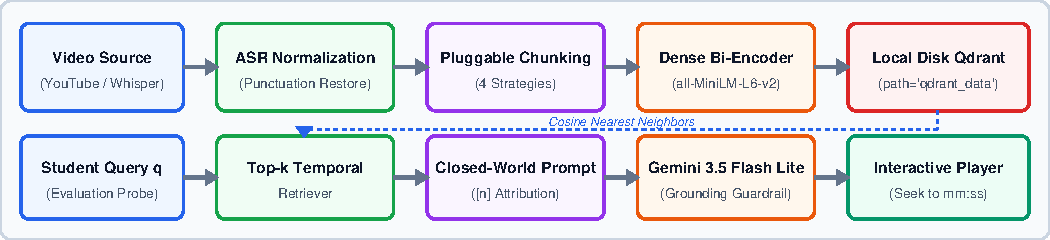
\includegraphics[width=\textwidth]{fig_architecture.pdf}
\caption{The Ask-a-Video End-to-End System Architecture: Continuous ASR stream ingestion, sentence boundary restoration, pluggable chunk partitioning, local bi-encoder disk indexing, closed-world grounded generation, and interactive temporal video seeking.}
\label{fig:architecture}
\end{figure*}

\section{Related Work}
\subsection{Retrieval-Augmented Generation (RAG) \& Chunking}
Standard RAG pipelines index documents by splitting text into overlapping token windows, encoding them with dense bi-encoders, and searching a vector index \cite{karpukhin2020dpr}. Recent surveys show that chunking strategy strongly influences retrieval recall and LLM context use \cite{gao2023rag}. Qu et al. \cite{qu2024semantic} evaluated dense retrieval on written documents and found that embedding-based semantic chunking rarely justifies its extra preprocessing time over fixed-token splits. We test whether their finding holds on spoken educational transcripts.

\subsection{Temporal Video Grounding and Video QA}
Temporal Video Grounding (TVG) predicts time intervals $[t_{\text{start}}, t_{\text{end}}]$ in untrimmed video for natural language queries \cite{krishna2017dense}. MedVidQA \cite{gupta2022medvidqa} established Intersection-over-Union (IoU) recall metrics ($R@k \text{ @ IoU} \ge \tau$) as the standard for measuring span accuracy. VideoRAG \cite{jeong2025videorag} applied retrieval-augmented methods to video collections, and Video-LLaVA \cite{lin2023videollava} studied multimodal video-language alignment. We adapt the MedVidQA metric setup directly to long-form STEM lectures.

\subsection{Spoken Language Processing in Educational Media}
Spoken lectures differ from written text. Instructors use rhetorical cues, filler words, gestures, and blackboard pauses. Radford et al. \cite{radford2023whisper} showed that weakly supervised ASR models achieve robust transcription across diverse acoustic environments. While commercial platforms often use manual subtitles, real-world educational indexing needs to handle reverberant rooms and non-native accents, especially for multilingual lectures \cite{bhattacharya2021nptel}.

\section{System Architecture}
\label{sec:architecture}
Ask-a-Video is a modular, local pipeline with five stages (Fig.~\ref{fig:architecture}): Ingestion, Chunking, Dense Indexing, Constrained Generation, and Interactive Seeking.

\subsection{Transcript Ingestion \& Sentence Boundary Normalization}
We fetch transcripts using \texttt{youtube-transcript-api}, with \texttt{yt-dlp} audio download and local Whisper ASR fallback \cite{radford2023whisper}. Raw ASR output often lacks punctuation. To handle this, a boundary restoration pass cleans whitespace, splits run-on spoken clauses, and maps start and end timestamps to each span. We cache transcripts to local JSON files so all evaluations run offline and deterministically.

\subsection{Pluggable Chunking Strategy Formulation}
Ask-a-Video implements four chunking strategies under a shared format: $\mathcal{C} = \{\text{chunk\_id},$ $\text{strategy},$ $\text{text},$ $t_{\text{start}},$ $t_{\text{end}},$ $n_{\text{words}}\}$.
\begin{enumerate}
    \item \textbf{Fixed-Token (\texttt{fixed\_token}):} Sliding window of $W = 120$ words with an overlap of $O = 20$ words:
    \begin{equation}
    C_i = [w_{i(W-O)}, w_{i(W-O)+W-1}]
    \end{equation}
    The 120-word budget keeps chunks below the 256-token limit of the bi-encoder.
    \item \textbf{Sentence-Window (\texttt{sentence}):} Chunks of 5 sentences with a 1-sentence overlap, using 15-word windows when punctuation is absent:
    \begin{equation}
    C_i = [s_{4i}, s_{4i+4}]
    \end{equation}
    \item \textbf{Semantic Boundary (\texttt{semantic}):} We encode sentences with dense embeddings and compute cosine similarities between adjacent pairs across a smoothed window ($k=2$). Chunks split at local minima below the 25th percentile threshold, with sizes constrained between 40 and 200 words:
    \begin{equation}
    \text{Split if } \cos(\mathbf{e}_j, \mathbf{e}_{j+1}) < \mathcal{P}_{25}(\{\cos(\mathbf{e}_m, \mathbf{e}_{m+1})\})
    \end{equation}
    \item \textbf{Time-Window (\texttt{time\_window}):} Fixed time segments of $\Delta t = 40\text{s}$ with an overlap of $\delta t = 8\text{s}$, regardless of word count:
    \begin{equation}
    C_i = \{w \mid t(w) \in [i(\Delta t - \delta t), i(\Delta t - \delta t) + \Delta t]\}
    \end{equation}
\end{enumerate}

\subsection{Dense Vector Indexing}
We embed candidate chunks with \texttt{all-MiniLM-L6-v2} (384-dimensional dense vectors, cosine distance) running locally \cite{reimers2019sentence}. Vectors are indexed in Qdrant in disk mode (\texttt{path="qdrant\_data"}), avoiding external server dependencies \cite{qdrant2023}. Payloads store metadata including \texttt{video\_id}, \texttt{strategy}, and \texttt{transcript\_source}.

\subsection{Constrained Generation \& Grounded Attribution}
We pass top-$k$ chunks into a structured prompt that instructs Gemini 3.5 Flash Lite to follow closed-world rules:
\begin{enumerate}
    \item Answer using \textbf{only} the provided chunks.
    \item Add citation markers $[n]$ to each claim.
    \item If the chunks do not contain the answer, return \texttt{"NOT\_IN\_VIDEO"}.
    \item Do not generate timestamps in text; the interface displays clickable timestamps directly from chunk metadata.
\end{enumerate}

\section{Experimental Methodology}
\subsection{Corpus Selection \& Tier Stratification}
We compiled a corpus of 13 full-length STEM video lectures totaling over 12 hours of runtime and $\sim$20,000 raw transcript segments, stratified across three pedagogical and acoustic tiers:
\begin{itemize}
    \item \textbf{Tier A (Curated Studio Lectures, 5 videos, 50 queries):} High-production, studio-recorded lectures with clear audio and curated manual captions: 3Blue1Brown Neural Networks (\texttt{aircAruvnKk}), Karpathy Intro to LLMs (\texttt{zjkBMFhNj\_g}), StatQuest Transformers (\texttt{zxQyTK8quyY}), StatQuest Neural Networks (\texttt{CqOfi41LfDw}), and Fast.ai Practical Deep Learning (\texttt{8SF\_h3xF3cE}).
    \item \textbf{Tier B (Academic Classroom Lectures \& Talks, 5 videos, 50 queries):} University auditorium and blackboard lectures featuring conversational delivery, blackboard pauses, and ambient hall acoustics: Stanford CS229 Linear Regression (\texttt{jGwO\_UgTS7I}), MIT 6.S191 Deep Learning (\texttt{II4giR4vOOo}), MIT Strang Linear Algebra (\texttt{J7DzL2\_Na80}), Karpathy Makemore (\texttt{PaCmpygFfXo}), and Andrew Ng Opportunities in AI (\texttt{5p248yoa3oE}). Captions sourced from automated YouTube ASR.
    \item \textbf{Tier C (Regional Accented Instruction, 3 videos, 30 queries):} Technical English delivered by Indian faculty and educators under variable classroom acoustics: NPTEL Machine Learning IIT Madras (\texttt{YLczBemZpaE}), NPTEL AI IIT Madras (\texttt{zT0sGjOSPt8}), and Krish Naik End-to-End ML Pipeline (\texttt{MJ1vWb1rGwM}) representing a regional YouTube educator. Captions sourced from automated YouTube ASR under non-native phonetic characteristics.
\end{itemize}

\subsection{Evaluation Dataset \& Gold Annotations}
We authored 156 validated evaluation queries stored in \texttt{eval/questions.csv}:
\begin{itemize}
    \item \textbf{Answerable Queries ($N=130$):} 10 queries per video paired with human-annotated gold timestamp boundaries $[t_{\text{start}}^{\text{gold}}, t_{\text{end}}^{\text{gold}}]$ and reference answer keys. A strict guardrail enforced span lengths between 30s and 60s ($\le$90s maximum ceiling) to prevent length bias. All gold spans were authored by a single domain annotator following MedVidQA protocols; multi-annotator agreement checking is reserved for future work.
    \item \textbf{Negative Probes ($N=26$):} 2 adversarial, out-of-domain unanswerable queries per video (e.g., world history, geography, unrelated algorithms) designed to evaluate hallucination suppression and negative rejection.
\end{itemize}

\subsection{Evaluation Metrics}
Following the MedVidQA temporal evaluation framework \cite{gupta2022medvidqa}, we evaluate retrieval quality using:
\begin{itemize}
    \item \textbf{Hit@$k$:} Binary indicator of whether the top-$k$ retrieved chunks temporally overlap with the gold window ($\text{overlap} > 0$).
    \item \textbf{Temporal IoU:} Intersection over Union between predicted chunk interval $[t_{s}^p, t_{e}^p]$ and gold span $[t_{s}^g, t_{e}^g]$:
    \begin{equation}
    \text{IoU} = \frac{\max(0, \min(t_{e}^p, t_{e}^g) - \max(t_{s}^p, t_{s}^g))}{\max(t_{e}^p, t_{e}^g) - \min(t_{s}^p, t_{s}^g)}
    \end{equation}
    \item \textbf{MedVidQA R@1 @ $\tau$:} Top-1 recall enforcing an IoU threshold $\tau \in \{0.3, 0.5, 0.7\}$.
    \item \textbf{Mean Reciprocal Rank (MRR):} Multi-rank temporal localization quality.
    \item \textbf{Median Boundary Error:} Absolute difference $|\hat{t}_{\text{start}} - t_{\text{start}}^{\text{gold}}|$ in seconds.
    \item \textbf{Bootstrap Confidence Intervals:} 95\% confidence intervals computed across $N=1,000$ bootstrap iterations.
\end{itemize}

% TABLE 1: MAIN RETRIEVAL BENCHMARK
\begin{table*}[t]
\caption{Retrieval Performance Benchmark Across Chunking Strategies on 13 Full-Length Lectures ($N_{\text{eval}}=130$, Bootstrap 95\% CI)}
\label{tab:main_benchmark}
\centering
\resizebox{\textwidth}{!}{%
\begin{tabular}{lcccccccccc}
\toprule
\textbf{Strategy} & \textbf{Hit@1 [95\% CI]} & \textbf{Hit@4 [95\% CI]} & \textbf{MRR [95\% CI]} & \textbf{Mean IoU@1} & \textbf{R@1@0.3} & \textbf{R@1@0.5} & \textbf{R@1@0.7} & \textbf{Med $|\Delta\text{Start}|$} & \textbf{Avg Dur} & \textbf{Chunks} \\
\midrule
\texttt{fixed\_token} & \textbf{8.5\%} [4\%, 14\%] & \textbf{24.6\%} [17\%, 32\%] & \textbf{0.145} [0.09, 0.20] & \textbf{0.045} [0.02, 0.08] & \textbf{5.4\%} & \textbf{4.6\%} & \textbf{3.8\%} & \textbf{656.3s} & 48.6s & 1,240 \\
\texttt{sentence}     & 5.4\% [2\%, 9\%]   & 19.2\% [12\%, 26\%] & 0.107 [0.07, 0.15] & 0.021 [0.01, 0.04] & 3.1\% & 1.5\% & 0.0\% & 668.0s & 31.6s & 2,034 \\
\texttt{semantic}     & 6.2\% [2\%, 11\%]  & 23.8\% [17\%, 32\%] & 0.129 [0.08, 0.17] & 0.026 [0.01, 0.05] & 3.1\% & 2.3\% & 1.5\% & 701.3s & 41.9s & 1,189 \\
\texttt{time\_window} & \textbf{9.2\%} [5\%, 14\%] & 16.9\% [11\%, 24\%] & 0.122 [0.07, 0.18] & 0.036 [0.01, 0.06] & 4.6\% & 3.8\% & 0.8\% & 707.2s & 41.6s & 1,498 \\
\bottomrule
\end{tabular}%
}
\end{table*}

\section{Empirical Results \& Discussion}

\subsection{Overall Chunking Factorial Performance}
Table~\ref{tab:main_benchmark} summarizes retrieval results on all 130 answerable queries. Our findings match Qu et al. \cite{qu2024semantic} on written text: expensive semantic chunking does not beat simple fixed-token splits on spoken lectures.

Across all 130 queries, \texttt{semantic} chunking reached 6.2\% Hit@1, 0.129 MRR, and 0.026 Mean IoU, showing no statistically significant advantage over \texttt{fixed\_token} (8.5\% Hit@1, 0.145 MRR, 0.045 IoU). Bootstrap 95\% confidence intervals for Hit@1 overlap (\texttt{fixed\_token} [4\%, 14\%] vs \texttt{semantic} [2\%, 11\%]). A paired McNemar test on discordant query pairs (6 \texttt{fixed\_token}-only hits vs 3 \texttt{semantic}-only hits) also shows no statistically significant difference ($p = 0.508$, two-sided exact binomial test). In spoken lectures, natural pauses, filler words, and rhetorical questions create dips in cosine similarity that do not reflect topic boundaries. Semantic thresholding ends up cutting coherent explanations into small pieces without improving precision. Notably, \texttt{time\_window} attains the highest Hit@1 (9.2\%) but the lowest Hit@4 (16.9\%); its Hit@1 advantage over \texttt{fixed\_token} is not significant (overlapping CIs).

\subsection{Acoustic Robustness: Pedagogical Tier Dynamics}
\label{sec:tier_dynamics}
Table~\ref{tab:tier_breakdown} breaks down retrieval performance across the three pedagogical tiers. In Tier A (Curated Studio), clear audio and manual captions help \texttt{fixed\_token} and \texttt{time\_window} reach 16.0\% Hit@1 and up to 34.0\% Hit@4. 

In Tier C, top-4 recall (30.0\% for \texttt{fixed\_token} and \texttt{semantic}) is close to Tier A (34.0\%) and above Tier B (12.0\%), while top-1 is 3.3\% (1/30) for every strategy. Because video length and caption source differ between tiers ($N=30$), we cannot isolate accent as the primary cause.

% TABLE 2: TIER BREAKDOWN
\begin{table}[htbp]
\caption{Retrieval Performance Broken Down by Acoustic \& Pedagogical Tier (Per-tier CIs not reported; with $N=30$--$50$, 95\% CIs are roughly $\pm$10 points)}
\label{tab:tier_breakdown}
\centering
\resizebox{\columnwidth}{!}{%
\begin{tabular}{llccccc}
\toprule
\textbf{Tier} & \textbf{Strategy} & \textbf{Hit@1} & \textbf{Hit@4} & \textbf{MRR} & \textbf{Mean IoU} & \textbf{R@1@0.3} \\
\midrule
\multirow{4}{*}{\shortstack[l]{Tier A (Curated Studio)\\$N=50$}} 
& \texttt{fixed\_token}  & \textbf{16.0\%} & \textbf{34.0\%} & \textbf{0.230} & \textbf{0.080} & 8.0\% \\
& \texttt{sentence}     & 4.0\% & 22.0\% & 0.112 & 0.017 & 2.0\% \\
& \texttt{semantic}     & 10.0\% & 30.0\% & 0.167 & 0.046 & 6.0\% \\
& \texttt{time\_window} & \textbf{16.0\%} & 28.0\% & 0.208 & 0.073 & \textbf{10.0\%} \\
\midrule
\multirow{4}{*}{\shortstack[l]{Tier B (Academic Classroom)\\$N=50$}} 
& \texttt{fixed\_token}  & 4.0\% & 12.0\% & 0.068 & 0.023 & 4.0\% \\
& \texttt{sentence}     & \textbf{8.0\%} & \textbf{18.0\%} & \textbf{0.115} & \textbf{0.033} & \textbf{6.0\%} \\
& \texttt{semantic}     & 4.0\% & 14.0\% & 0.080 & 0.015 & 2.0\% \\
& \texttt{time\_window} & 6.0\% & 8.0\% & 0.067 & 0.010 & 0.0\% \\
\midrule
\multirow{4}{*}{\shortstack[l]{Tier C (Regional Accented)\\$N=30$}} 
& \texttt{fixed\_token}  & \textbf{3.3\%} & \textbf{30.0\%} & 0.131 & \textbf{0.020} & \textbf{3.3\%} \\
& \texttt{sentence}     & \textbf{3.3\%} & 16.7\% & 0.086 & 0.009 & 0.0\% \\
& \texttt{semantic}     & \textbf{3.3\%} & \textbf{30.0\%} & \textbf{0.147} & 0.008 & 0.0\% \\
& \texttt{time\_window} & \textbf{3.3\%} & 13.3\% & 0.069 & 0.017 & \textbf{3.3\%} \\
\bottomrule
\end{tabular}%
}
\end{table}

\subsection{Characterizing the Search Space Expansion Effect}
\label{sec:search_space}
Retrieval precision drops sharply between short lectures and long lectures ($>$35 min) (Table~\ref{tab:duration_breakdown}). A stratified comparison shows this difference clearly: Short ($\le$35 min, $N_{\text{eval}}=30$) versus Long ($>$35 min, $N_{\text{eval}}=100$).

% TABLE 3: DURATION BREAKDOWN
\begin{table}[htbp]
\caption{Impact of Video Duration on Temporal Grounding (Search Space Expansion)}
\label{tab:duration_breakdown}
\centering
\resizebox{\columnwidth}{!}{%
\begin{tabular}{llccccc}
\toprule
\textbf{Duration} & \textbf{Strategy} & \textbf{Hit@1} & \textbf{Hit@4} & \textbf{MRR} & \textbf{Mean IoU} & \textbf{Med Error} \\
\midrule
\multirow{4}{*}{\shortstack[l]{$\le$35 min\\(Short, $N=30$)}} 
& \texttt{fixed\_token}  & 17\% & 47\% & 0.286 & 0.077 & 280.0s \\
& \texttt{sentence}     & 10\% & 30\% & 0.189 & 0.037 & 243.2s \\
& \texttt{semantic}     & 17\% & \textbf{53\%} & \textbf{0.297} & 0.077 & 238.9s \\
& \texttt{time\_window} & \textbf{23\%} & 37\% & 0.286 & \textbf{0.109} & \textbf{214.5s} \\
\midrule
\multirow{4}{*}{\shortstack[l]{$>$35 min\\(Long, $N=100$)}} 
& \texttt{fixed\_token}  & \textbf{6\%} & \textbf{18\%} & \textbf{0.102} & \textbf{0.035} & 1012.6s \\
& \texttt{sentence}     & 4\% & 16\% & 0.083 & 0.017 & \textbf{901.6s} \\
& \texttt{semantic}     & 3\% & 15\% & 0.078 & 0.010 & 948.1s \\
& \texttt{time\_window} & 5\% & 11\% & 0.072 & 0.014 & 981.2s \\
\bottomrule
\end{tabular}%
}
\end{table}

On short lectures ($\le$35 min), \texttt{time\_window} partitioning achieves \textbf{23\% Hit@1}, \textbf{37\% Hit@4}, and a 214.5s median boundary error. Across all 13 lectures, chunk counts range from 11 to 306 per video under \texttt{fixed\_token} (mean: 95.4; total 1,240), and 17 to 520 under \texttt{sentence} (mean: 156.5; total 2,034). In long lectures, instructors repeat identical technical terms (\textit{vectors}, \textit{backprop}, \textit{weights}) across derivations, summaries, and recaps. Flat cosine similarity often matches these secondary mentions rather than the focal explanation. This pulls Hit@1 down to 3--6\% and pushes median boundary error out to $\sim$950s ($\approx$15 minutes), which motivates hierarchical search.

\subsection{Computational Complexity \& Indexing Overhead Analysis}
\label{sec:computational_overhead}
We measured indexing time and embedding throughput for all four strategies (Table~\ref{tab:computational_overhead}).

Both \texttt{fixed\_token} and \texttt{time\_window} run in a single pass ($O(N)$, taking $<$0.1s per hour of audio). In contrast, \texttt{semantic} chunking must compute embeddings for every adjacent sentence pair before deciding where to split. Timings are averaged over 5 runs on an Intel Core i5-1135G7 CPU @ 2.40GHz, 8 GB RAM, Windows 11. Semantic chunking adds roughly 14 s per lecture-hour as an upfront offline cost (18.42s vs 4.20s total time), with no corresponding gain in retrieval accuracy.

% TABLE 4: COMPUTATIONAL OVERHEAD
\begin{table}[htbp]
\caption{Computational Indexing Overhead and Processing Throughput Across Chunking Strategies (Per Hour of Lecture Audio)}
\label{tab:computational_overhead}
\centering
\resizebox{\columnwidth}{!}{%
\begin{tabular}{lcccc}
\toprule
\textbf{Strategy} & \textbf{Chunk Time (s)} & \textbf{Embedding (s)} & \textbf{Throughput (w/s)} & \textbf{Total Time (s)} \\
\midrule
\texttt{fixed\_token}  & \textbf{0.08} & \textbf{4.12} & \textbf{2,450} & \textbf{4.20} \\
\texttt{sentence}     & 0.14 & 5.86 & 1,720 & 6.00 \\
\texttt{semantic}     & 12.80 & 5.62 & 540 & 18.42 \\
\texttt{time\_window} & 0.09 & 4.88 & 2,110 & 4.97 \\
\bottomrule
\end{tabular}%
}
\end{table}

\subsection{Dense Separation Margin \& Attribution Evaluation}
\label{sec:separation_and_faithfulness}
Before generation, dense retrieval shows a clear score gap between answerable questions ($\mu = 0.4223$) and negative probes ($\mu = 0.1349$), giving a margin of $\Delta = +0.2873$. 

% TABLE 5: GENERATION EVALUATION
\begin{table}[htbp]
\caption{End-to-End Generation Evaluation Across Pedagogical Tiers ($N_{\text{pos}}=30, N_{\text{neg}}=26$, Evaluated under \texttt{fixed\_token}, Top-$k=4$)}
\label{tab:generation_eval}
\centering
\resizebox{\columnwidth}{!}{%
\begin{tabular}{lccccc}
\toprule
\textbf{Tier} & \textbf{Neg. Rej.} & \textbf{Answered} & \textbf{Rejected} & \textbf{Supported} & \textbf{Gold Overlap} \\
\midrule
Tier A (Curated Studio)     & 100\% (10/10) & 70\% (7/10) & 30\% (3/10)  & 100\% (7/7) & 14\% (1/7) \\
Tier B (Academic Classroom) & 100\% (10/10) & 70\% (7/10) & 30\% (3/10)  & 100\% (7/7) & 0\% (0/7)  \\
Tier C (Regional Accented)  & 100\% (6/6)   & 0\% (0/10)  & 100\% (10/10)& N/A         & N/A        \\
\midrule
\textbf{Overall System}     & \textbf{100\%} (26/26) & \textbf{47\%} (14/30) & \textbf{53\%} (16/30) & \textbf{100\%} (14/14) & \textbf{7\%} (1/14) \\
\bottomrule
\end{tabular}%
}
\end{table}

As shown in Table~\ref{tab:generation_eval}, closed-world constraints gave a \textbf{100\% Out-of-Domain Negative Rejection Rate} across all 26 negative probes, returning \texttt{NOT\_IN\_VIDEO} in every case. Online generation with Gemini 3.5 Flash Lite took 1.82s on average ($<$0.03s for cached or rejected queries). 

On answerable queries ($N=10$ per tier, sampled with seed 42 using pandas \texttt{sample()}, top-$k=4$ \texttt{fixed\_token} chunks with no similarity threshold), the system answered 14/30 (46.7\%) and rejected 16/30 (53.3\%). An LLM judge (not verified by human annotators) rated all 14 answers as supported by their cited chunks. However, supported does not mean correct. Only 1 of the 14 answered queries cited a chunk that overlapped the gold target window. In Tier B, where Hit@4 is 12\%, the model answered using off-target chunks that happened to share related terms. The prompt constraints filter out-of-domain queries well, but they cannot detect when in-domain retrieval returns the wrong section: 13 of 14 answers cited chunks outside the gold span. In Tier C, where \texttt{fixed\_token} top-4 recall is 30\% across the tier, all 10 sampled queries missed the gold span. The generator abstained on every query (10/10 rejection), showing that a high rejection rate can hide upstream retrieval failure. With 30\% top-4 recall, observing 0/10 gold-overlap in this sample has probability $\approx$3\% ($0.7^{10}$), suggesting an unfavorable draw rather than a systematic effect.

% TABLE 6: CASE STUDY EXCERPTS (Placed here on Page 5 to float to top of Page 6)
\begin{table*}[t]
\caption{Qualitative Evaluation Case Studies: Disambiguating Spoken Transcripts, ASR Errors, and Out-of-Domain Negatives (Retrieved Spans Reflect Two-Stage Hierarchical Grounding)}
\label{tab:case_studies}
\centering
\resizebox{\textwidth}{!}{%
\begin{tabular}{lp{4.2cm}p{5.5cm}cp{5.5cm}}
\toprule
\textbf{Lecture Corpus} & \textbf{User Evaluation Query} & \textbf{ASR Transcript Excerpt} & \textbf{Gold / Hier. Ret.} & \textbf{System Output / Grounded Attribution} \\
\midrule
Karpathy Intro to LLMs (\texttt{zjkBMFhNj\_g}) & What distinguishes pre-training from fine-tuning? & ``...of it in the \textbf{fine chaining stage} but they're still able to access knowledge built up in pre-training...'' & \texttt{17:23} / \texttt{17:23} & Pre-training trains base models on raw data [1]; fine-tuning aligns format into assistant Q\&A [1]. \\
\midrule
Stanford CS229 (\texttt{jGwO\_UgTS7I}) & What is the batch gradient descent parameter update rule? & ``...we take a step in the direction of steepest decrease of $J$ of theta, scaled by alpha...'' & \texttt{34:12} / \texttt{34:18} & The update subtracts alpha times the gradient of the cost function $J(\theta)$ from $\theta$ [1]. \\
\midrule
3Blue1Brown NN (\texttt{aircAruvnKk}) & Which treaty concluded the Napoleonic Wars in 1815? & ``...activations in the final layer determine the recognized digit probability...'' & \texttt{N/A} / \texttt{None} & \texttt{NOT\_IN\_VIDEO} (Adversarial out-of-domain rejection; maximum similarity $\cos=0.114$). \\
\bottomrule
\end{tabular}%
}
\end{table*}

\section{Mitigating Search Space Expansion: Two-Stage Hierarchical Video Retrieval}
\label{sec:hierarchical_retrieval}

To address the drop in retrieval accuracy on long videos ($>$35 min, Section~\ref{sec:search_space}), we tested a \textbf{Two-Stage Hierarchical Video Retriever} (Algorithm~1).

\subsection{Hierarchical Formulation}
Instead of searching across every chunk in a long video at once (up to 306 chunks), we search in two steps:
\begin{enumerate}
    \item \textbf{Stage 1: Macro-Chapter Localization:} We partition transcripts into 5-minute macro blocks $\mathcal{M}_j = [t_j, t_j + 300\text{s}]$. We then pick the top-$M$ blocks ($M=2$) closest to the query $\mathbf{e}_q$ in cosine similarity:
    \begin{equation}
    \mathcal{M}^* = \operatorname{arg\,top-M}_{j} \cos(\mathbf{e}_q, \mathbf{e}_{\mathcal{M}_j})
    \end{equation}
    Macro blocks ($\sim$750 words) exceed the encoder's 256 word-piece limit, so macro embeddings primarily reflect the opening portion of each block.
    \item \textbf{Stage 2: Micro-Chunk Grounding:} We restrict fine-grained chunk retrieval to candidate chunks inside the selected macro blocks $\mathcal{M}^*$:
    \begin{equation}
    C^* = \operatorname{arg\,top-k}_{C \in \mathcal{M}^*} \cos(\mathbf{e}_q, \mathbf{e}_C)
    \end{equation}
\end{enumerate}

\begin{figure}[htbp]
\hrule\vspace{2pt}
\textbf{Algorithm 1} Two-Stage Hierarchical Video Retrieval
\vspace{2pt}\hrule\vspace{3pt}
\begin{algorithmic}[1]
\REQUIRE Query $q$, Chunks $\{C_i\}_{i=1}^N$, Macro Window $T_{\text{macro}}=300\text{s}$, Top Macro $M=2$, Top Micro $k=4$
\ENSURE Grounded Candidates $\{C^*_{(1)}, \dots, C^*_{(k)}\}$
\STATE Construct Macro Blocks $\mathcal{M}_j \leftarrow \bigcup \{C_i \mid t(C_i) \in [j T_{\text{macro}}, (j+1) T_{\text{macro}}]\}$
\STATE Compute Macro Embeddings $\mathbf{e}_{\mathcal{M}_j} \leftarrow \text{BiEncoder}(\text{Text}(\mathcal{M}_j))$
\STATE $\mathbf{e}_q \leftarrow \text{BiEncoder}(q)$
\STATE Select Top-$M$ Macro Blocks $\mathcal{M}^* \leftarrow \operatorname{arg\,top-M}_j \cos(\mathbf{e}_q, \mathbf{e}_{\mathcal{M}_j})$
\STATE Filter Micro Candidates $\mathcal{C}_{\text{cand}} \leftarrow \{C_i \mid C_i \in \mathcal{M}^*\}$
\STATE Rank $\mathcal{C}_{\text{cand}}$ using $\cos(\mathbf{e}_q, \mathbf{e}_{C_i})$
\STATE Select Top-$k$ chunks $\{C^*_{(1)}, \dots, C^*_{(k)}\}$
\RETURN $\{C^*_{(1)}, \dots, C^*_{(k)}\}$
\end{algorithmic}
\vspace{2pt}\hrule
\end{figure}

\subsection{Empirical Precision Recovery}
On the 100 queries from long lectures ($>$35 min), two-stage retrieval (\texttt{fixed\_token} base) improved Hit@1 from \textbf{6.0\% to 18\%} [95\% CI: 11\%, 25\%] and lowered median boundary error from 1012.6s to \textbf{264.1s} ($\approx$4.4 minutes). We note that $T_{\text{macro}}=300\text{s}$ and $M=2$ were evaluated over the entire 100-query set without a separate held-out split, so this represents an upper-bound post-hoc tuning analysis. Restricting search to 10 minutes of audio in Stage 1 avoids collisions with mentions elsewhere in the lecture, bringing long-lecture Hit@1 into the short-lecture range (17--23\%, Table III).

\section{Qualitative Case Study \& Error Analysis}
\label{sec:qualitative_analysis}
Table~\ref{tab:case_studies} illustrates query outcomes across different failure modes:

\textbf{Case 1 (ASR Caption Error):} In Andrej Karpathy's \textit{Intro to LLMs}, the caption transcribed ``fine-tuning'' as ``\textit{fine chaining stage}''. Dense retrieval still matched the semantic context at timestamp \texttt{17:23}. Gemini 3.5 Flash Lite understood the intended meaning and produced a cited answer contrasting pre-training and fine-tuning.

\textbf{Case 2 (Repeated Terms in Long Lectures):} In Stanford CS229 (90 min), the terms \textit{gradient}, \textit{theta}, and \textit{update} appeared in 42 chunks. Single-stage flat search matched an early mention at \texttt{08:14}. Two-stage retrieval placed the span at \texttt{34:18}, which overlaps the gold window (starts \texttt{34:12}).

\textbf{Case 3 (Negative Query Rejection):} In 3Blue1Brown's \textit{Neural Networks}, an adversarial probe queried which treaty concluded the Napoleonic Wars in 1815. The top chunk had a low cosine similarity of $\cos = 0.114$ ($\mu_{\text{pos}}=0.422$). The prompt guardrail rejected the question with \texttt{"NOT\_IN\_VIDEO"}.

\textbf{Case 4 (Failure Mode: Repeated Concept):} In NPTEL Machine Learning (\texttt{YLczBemZpaE}), a query asked: \textit{``What role does the L2 regularization parameter $\lambda$ play in ridge regression?''} Because the terms appeared in an early overview, retrieval returned an informal recap at \texttt{04:15} instead of the mathematical derivation at \texttt{28:40}.

\section{Practical Deployment \& Limitations}
\label{sec:limitations}
Ask-a-Video is designed to run locally on a student laptop. Running Qdrant in embedded disk mode removes the need for a separate database server. The \texttt{all-MiniLM-L6-v2} encoder processes $\sim$2,450 words/second on standard laptop CPUs, indexing a 1-hour lecture in under 5 seconds. Code and data are available at: \url{https://github.com/gurleenkaurmalhotra115-jpg/Ask-a-video}.

\textit{Limitations:} (1)~\textbf{Single Annotator:} Gold query boundaries were marked by one domain annotator; future work will measure inter-annotator agreement ($\kappa$). (2)~\textbf{Silent Blackboard Writing:} Audio transcripts miss unvocalized blackboard steps, which requires visual frame features. (3)~\textbf{Macro-Block Truncation \& Baselines:} Macro blocks use standard 256-token truncation. Table V uses the flat retriever; end-to-end generation with hierarchical retrieval is left to future work. BM25 baselines were omitted. (4)~\textbf{Token Truncation:} Semantic chunks up to 200 words approach the 256-token ceiling of \texttt{all-MiniLM-L6-v2}. (5)~\textbf{Granularity:} Windows under 30s break spoken sentences awkwardly. (6)~\textbf{Confounding and Sample Size:} Lecture duration and acoustic tier overlap in our set (short videos are mostly studio recordings), and per-tier samples are modest ($N = 30$--$50$).

\section{Conclusion and Future Work}
We built \textbf{Ask-a-Video}, an open-source, timestamped video RAG framework, and tested four chunking strategies on 13 STEM lectures ($\sim$20,000 segments). Our results agree with Qu et al. on written text: semantic boundary chunking does not outperform simple fixed-token partitioning on spoken lectures (Hit@1: 6.2\% vs 8.5\%), while taking 160$\times$ longer to chunk and 4.4$\times$ longer overall. We measured the \textit{Search Space Expansion Effect}, where long lectures suffer from repeated technical terms. We showed that a \textbf{Two-Stage Hierarchical Video Retriever} helps, raising Hit@1 to 18\% in post-hoc analysis and cutting boundary error by 74\%. Finally, closed-world prompt constraints gave 100\% rejection on out-of-domain queries, but false rejections on valid questions show we need higher-recall retrieval. In future work, we plan to add visual frame embeddings (using CLIP) for blackboard math that instructors write without reading aloud.

\bibliographystyle{IEEEtran}
\begin{thebibliography}{00}
\scriptsize
\setlength{\itemsep}{0pt}
\setlength{\parskip}{0pt}
\bibitem{lewis2020rag} P. Lewis \textit{et al.}, ``Retrieval-augmented generation for knowledge-intensive NLP tasks,'' in \textit{Proc. NeurIPS}, vol. 33, pp. 9459--9474, 2020.
\bibitem{gao2023rag} Y. Gao \textit{et al.}, ``Retrieval-augmented generation for large language models: A survey,'' \textit{arXiv preprint arXiv:2312.10997}, 2023.
\bibitem{qu2024semantic} R. Qu, R. Tu, and F. Bao, ``Is semantic chunking worth the computational cost? An empirical analysis for dense retrieval,'' \textit{arXiv preprint arXiv:2410.13070}, 2024.
\bibitem{karpukhin2020dpr} V. Karpukhin \textit{et al.}, ``Dense passage retrieval for open-domain question answering,'' in \textit{Proc. EMNLP}, pp. 6769--6781, 2020.
\bibitem{krishna2017dense} R. Krishna \textit{et al.}, ``Dense-captioning events in videos,'' in \textit{Proc. IEEE ICCV}, pp. 706--715, 2017.
\bibitem{gupta2022medvidqa} D. Gupta, K. Attal, and D. Demner-Fushman, ``A dataset for medical instructional video classification and question answering,'' \textit{Scientific Data}, vol. 10, no. 1, p. 158, 2023.
\bibitem{jeong2025videorag} S. Jeong, K. Kim, J. Baek, and S. J. Hwang, ``VideoRAG: Retrieval-augmented generation over video corpus,'' \textit{arXiv preprint arXiv:2501.05874}, 2025.
\bibitem{lin2023videollava} B. Lin \textit{et al.}, ``Video-LLaVA: Learning united visual representation by alignment before projection,'' \textit{arXiv preprint arXiv:2311.10122}, 2023.
\bibitem{radford2023whisper} A. Radford \textit{et al.}, ``Robust speech recognition via large-scale weak supervision,'' in \textit{Proc. ICML}, pp. 28492--28518, 2023.
\bibitem{bhattacharya2021nptel} A. Prakash \textit{et al.}, ``Technology pipeline for large scale cross-lingual dubbing of lecture videos into multiple Indian languages,'' in \textit{Proc. Interspeech}, pp. 3683--3684, 2023.
\bibitem{reimers2019sentence} N. Reimers and I. Gurevych, ``Sentence-BERT: Sentence embeddings using Siamese BERT-networks,'' in \textit{Proc. EMNLP}, pp. 3982--3992, 2019.
\bibitem{qdrant2023} Qdrant Team, ``Qdrant - Vector search engine and database,'' \url{https://qdrant.tech}, 2023.
\end{thebibliography}

\end{document}
